\section{Apache with mod\_php}

The first step is to compare the performance of Apache and Nginx web serving software. However, it is not necessary to compare these software in their speed of serving static content (for example HTML files) because it has been proven and because of Nginx architecture that Nginx is more performant in this manner.

What is interesting to compare, though, is running of PHP under Apache and Nginx.

Apache has a process-based architecture. When a request is sent, Apache starts to process it one by one, gradually. It spawns multiple threads to handle larger number of requests. However, these threads are standalone processes which have to load all settings and modules so they are usually taking a large amounts of RAM.

In most cases, PHP is loaded as Apache module. It has the advantage of being loaded directly into the thread, not needing to relay the request further. Disadvantages are that even if the request is for a static resource such as CSS or JS file, Apache loads all modules, including mod\_php for this. RAM and CPU usage therefore increases.

\begin{figure}[H]
\begin{center}
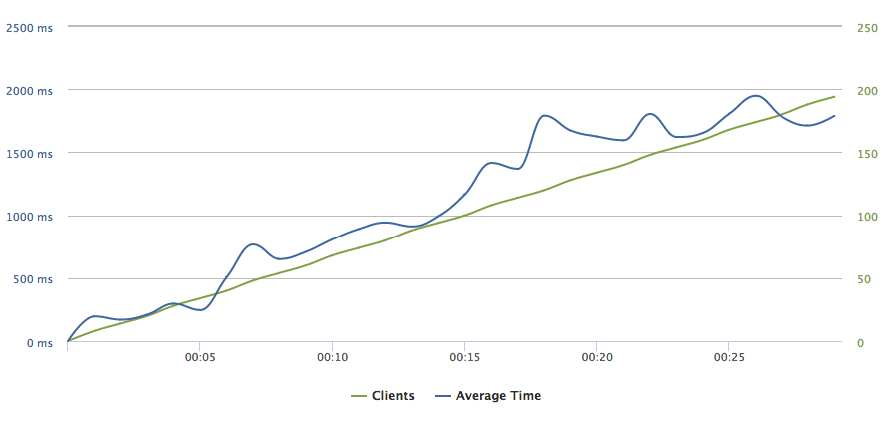
\includegraphics[scale=0.5]{figures/Apache_mod_php.png}
\caption{Apache HTTP with mod\_php: clients versus average response time}
\label{fig:apache_mod_php}
\end{center}
\end{figure}

\begin{figure}[H]
\begin{center}
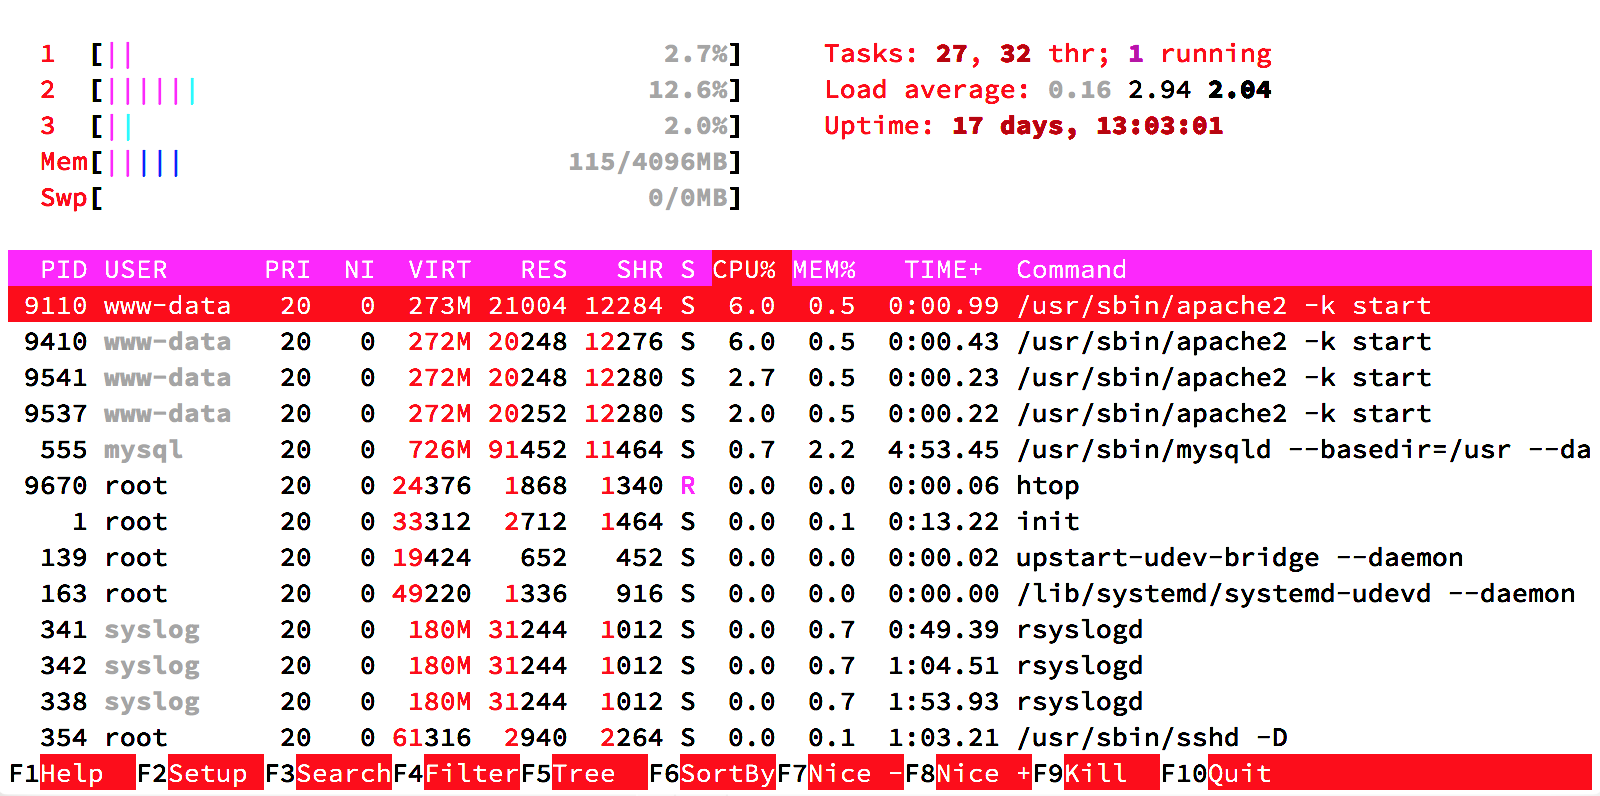
\includegraphics[scale=0.5]{figures/Apache_mod_php_2s.png}
\caption{Apache HTTP with mod\_php: Htop process viewer 2 seconds into test}
\label{fig:apache_mod_php_2s}
\end{center}
\end{figure}

\begin{figure}[H]
\begin{center}
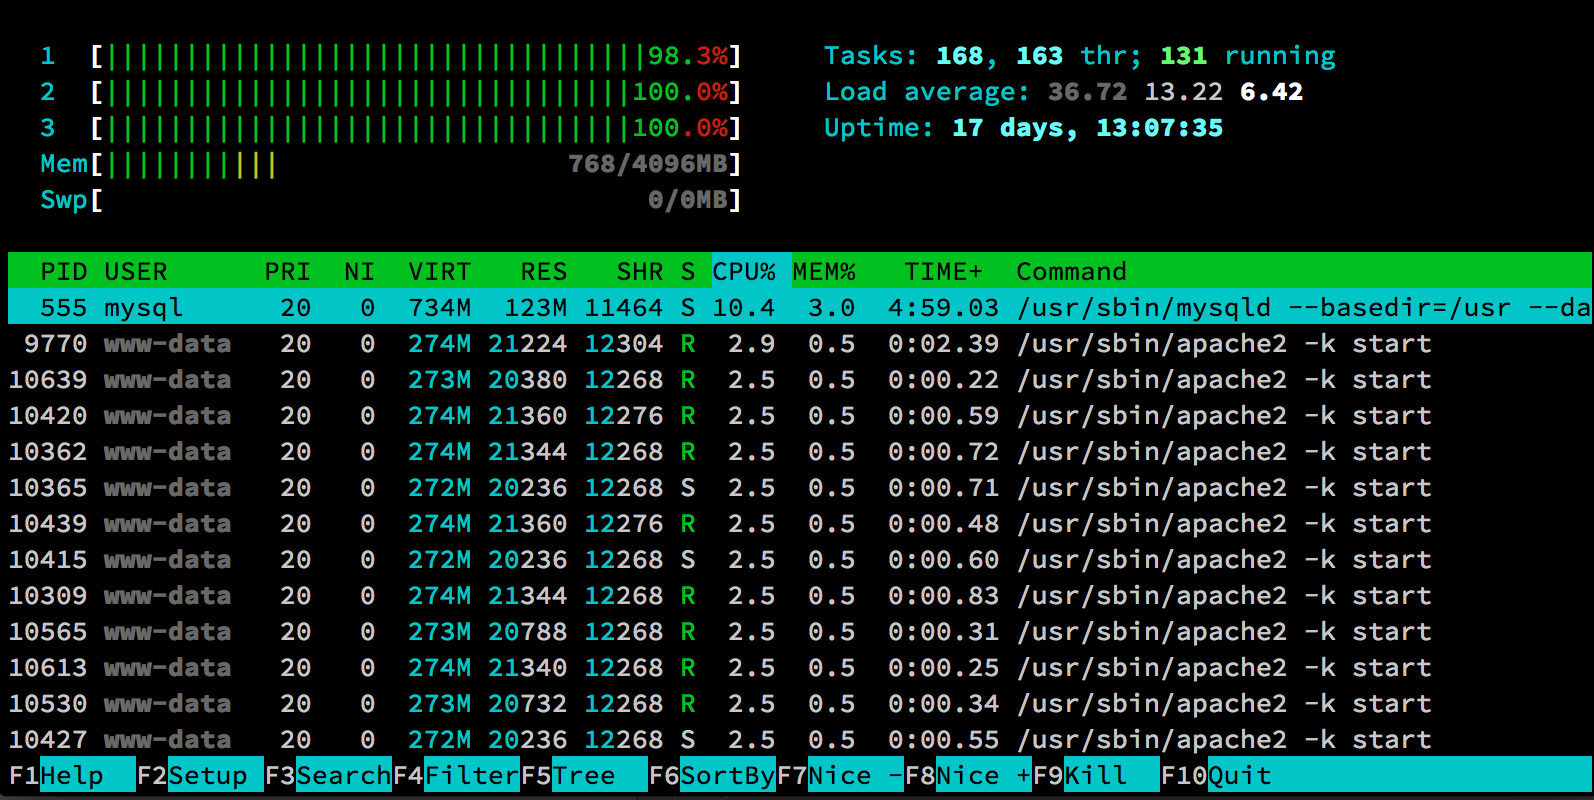
\includegraphics[scale=0.5]{figures/Apache_mod_php_25s.png}
\caption{Apache HTTP with mod\_php: Htop process viewer 25 seconds into test}
\label{fig:apache_mod_php_25s}
\end{center}
\end{figure}

As you can see from the graphs, Apache with mod\_php is performing quite well, surpassing Nginx with PHP-FPM. However, when we look at the server resources usage, we can see that RAM and CPU usage is much higher in Apache than in Nginx with PHP-FPM.

It is therefore better to use Nginx and PHP-FPM than Apache and mod\_php as your server web serving software. Nginx is not the bottleneck here, PHP-FPM is.

Has to switch to using TCP/IP to bypass server open file descriptors limitation which was slowing it down (sockets connection failed).

Include successful response count (= how many requests can it actually handle).

\section{Nginx with PHP-FPM}

Nginx has an event-based architecture. It means that when an request arrives, Nginx asynchronously listens for it. Then when it arrives, it is processed asynchronously. The main usage for Nginx is to quickly process many requests, relaying them to other applications if they need to be processed further. That's why we need to use PHP-FPM.

PHP-FPM is a FastCGI server bound to a TCP port or socket. It listens for PHP requests, processing them and outputting the rendered content.

When using Ningx with PHP, we have to detect if the request is for a PHP file. If it is, we need to redirect the request into the PHP-FPM server, waiting for the reply which is then outputted as a response.


To compare Apache with mod\_php and Nginx with PHP-FPM, they are similarly performant. Apache + mod\_php can achieve better performance at the expense of wasting more resources as it has to spawn a large number of threads to process more requests. 

\begin{figure}[H]
\begin{center}
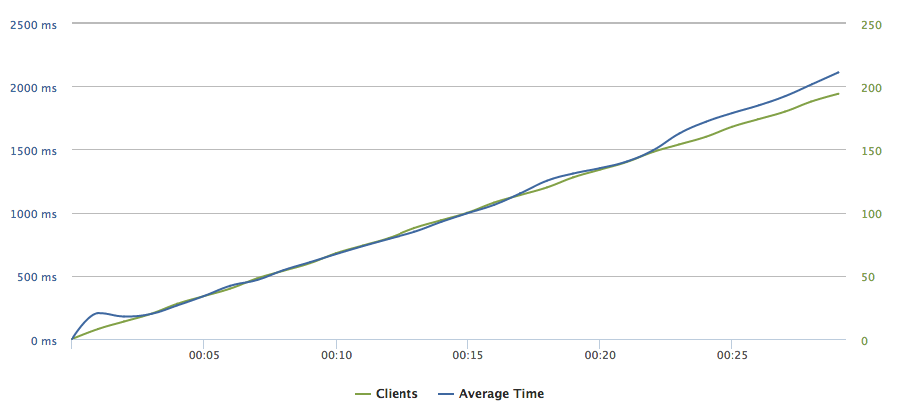
\includegraphics[scale=0.5]{figures/Nginx_PHP-FPM.png}
\caption{Nginx with PHP-FPM: clients versus average response time}
\label{fig:nginx_php-fpm}
\end{center}
\end{figure}

\begin{figure}[H]
\begin{center}
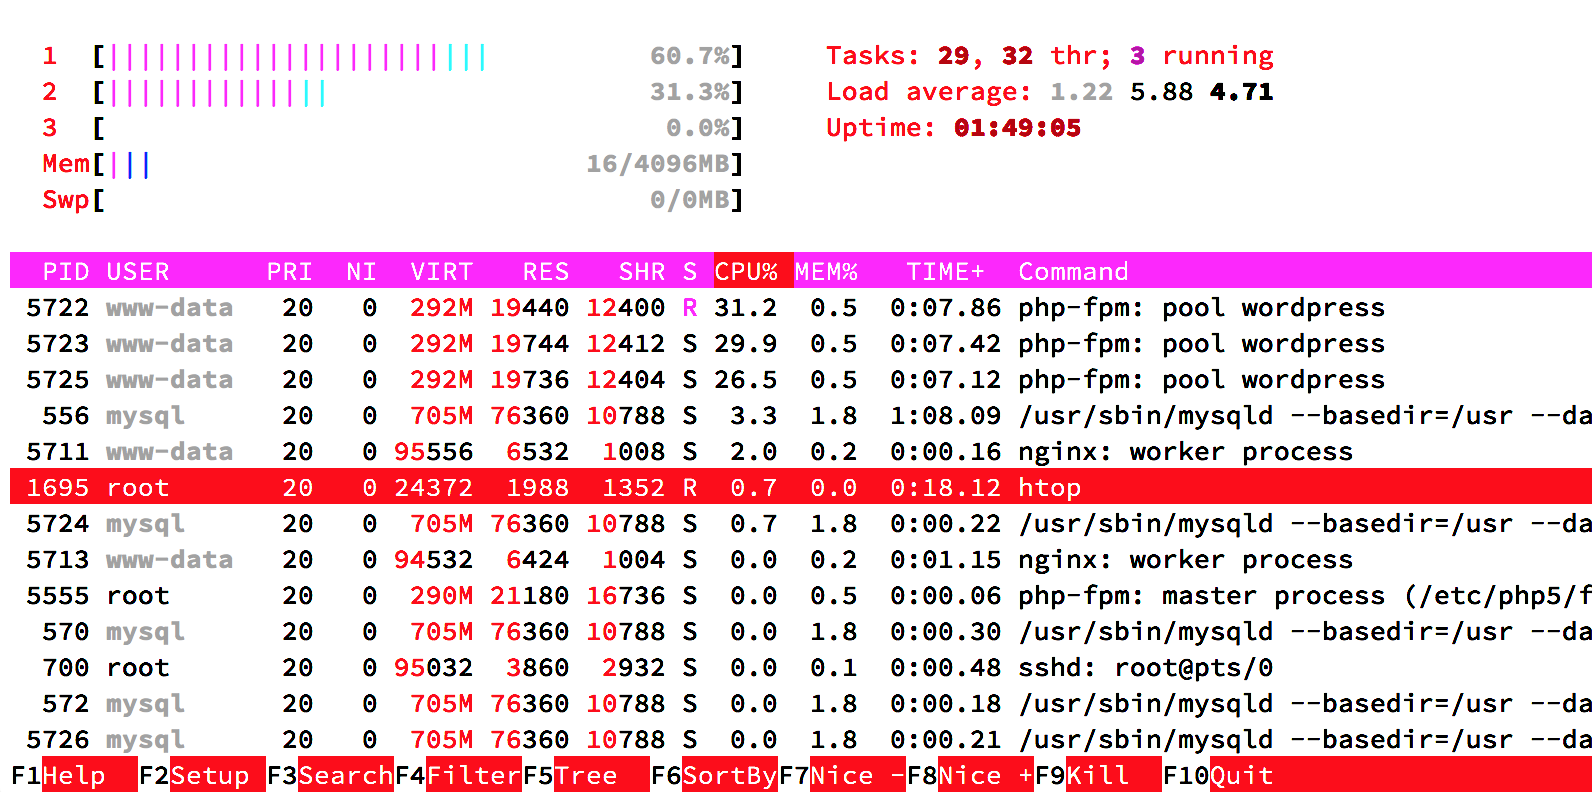
\includegraphics[scale=0.5]{figures/Nginx_PHP-FPM_1s.png}
\caption{Nginx with PHP-FPM: Htop process viewer 1 second into test}
\label{fig:nginx_php-fpm_1s}
\end{center}
\end{figure}

\begin{figure}[H]
\begin{center}
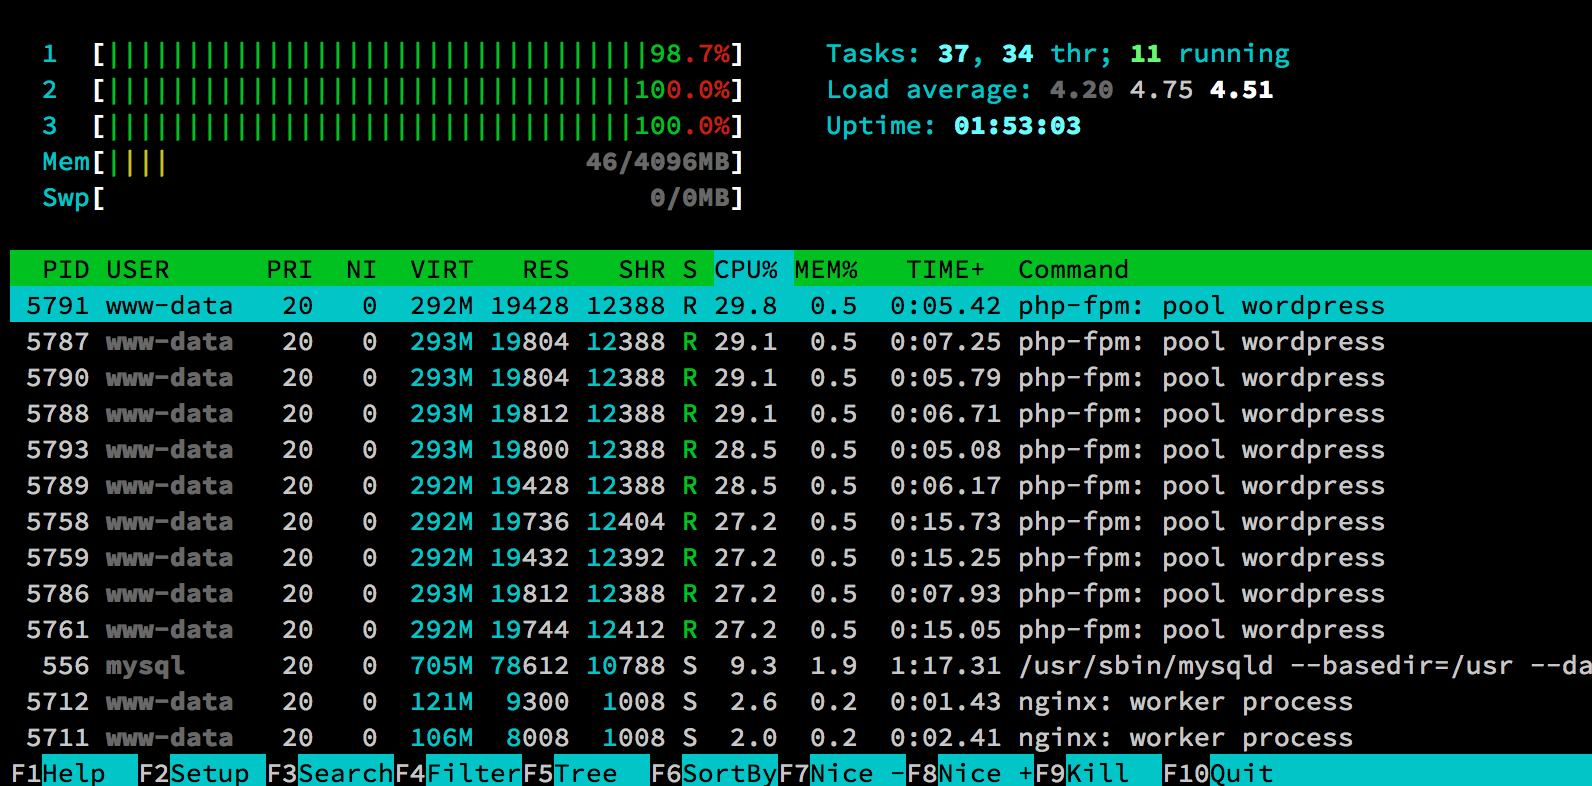
\includegraphics[scale=0.5]{figures/Nginx_PHP-FPM_22s.png}
\caption{Nginx with PHP-FPM: Htop process viewer 22 seconds into test}
\label{fig:nginx_php-fpm_22s}
\end{center}
\end{figure}

\section{Nginx + HHVM}

In the previous section, we have seen the performance of Nginx + PHP-FPM. Now, we will compare it with Nginx using HHVM for PHP processsing.

"HipHop Virtual Machine (HHVM) is a process virtual machine based on just-in-time (JIT) compilation, serving as an execution engine for PHP...". "By using the principle of JIT compilation, executed PHP or Hack code is first transformed into intermediate HipHop bytecode (HHBC), which is then dynamically translated into the x86-64 machine code, optimized and natively executed.[1][4] This contrasts to the PHP's usual interpreted execution, in which the Zend Engine transforms the PHP source code into opcodes as a form of intermediate code, and executes the opcodes directly on the Zend Engine's virtual CPU".

It is developed by Facebook with source code hosted on GitHub (open source).

\begin{figure}[H]
\begin{center}
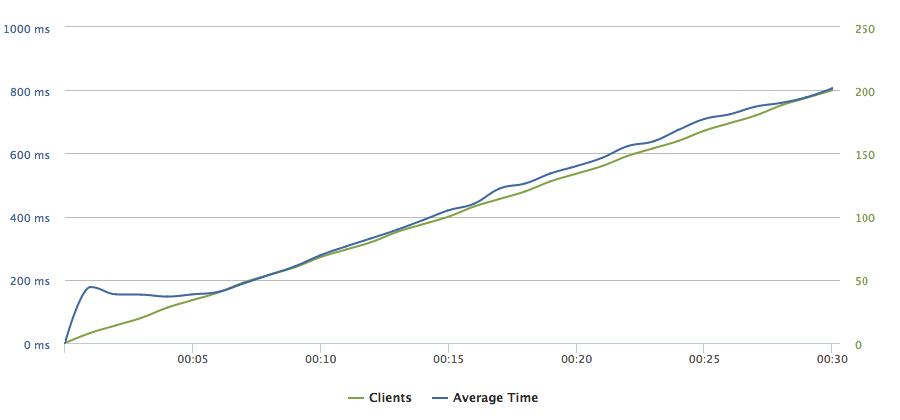
\includegraphics[scale=0.5]{figures/Nginx_HHVM.png}
\caption{Nginx with HHVM: clients versus average response time}
\label{fig:nginx_hhvm}
\end{center}
\end{figure}

\begin{figure}[H]
\begin{center}
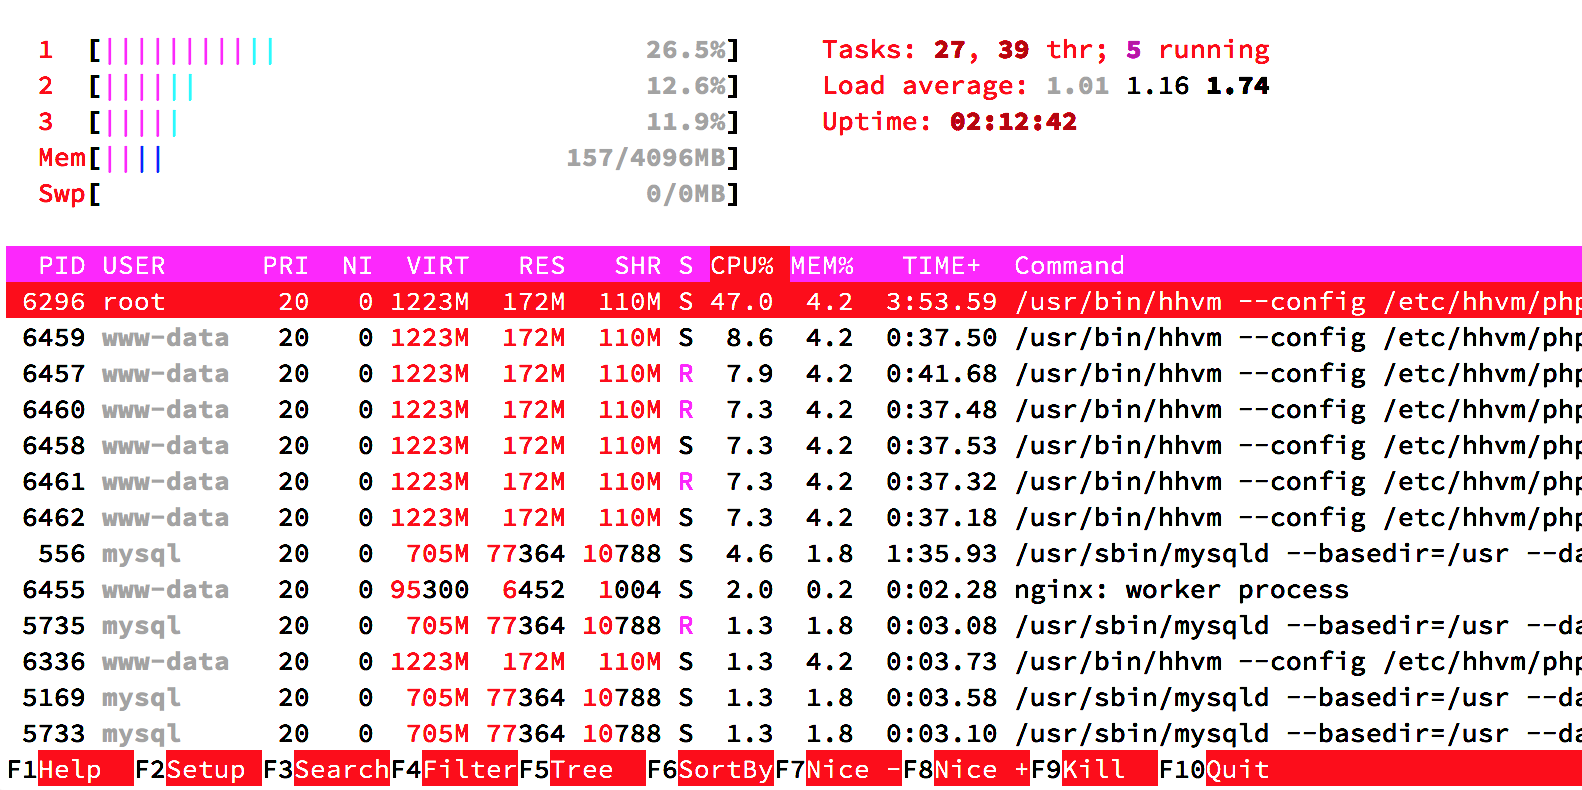
\includegraphics[scale=0.5]{figures/Nginx_HHVM_1s.png}
\caption{Nginx with HHVM: Htop process viewer 1 second into test}
\label{fig:nginx_hhvm_1s}
\end{center}
\end{figure}

\begin{figure}[H]
\begin{center}
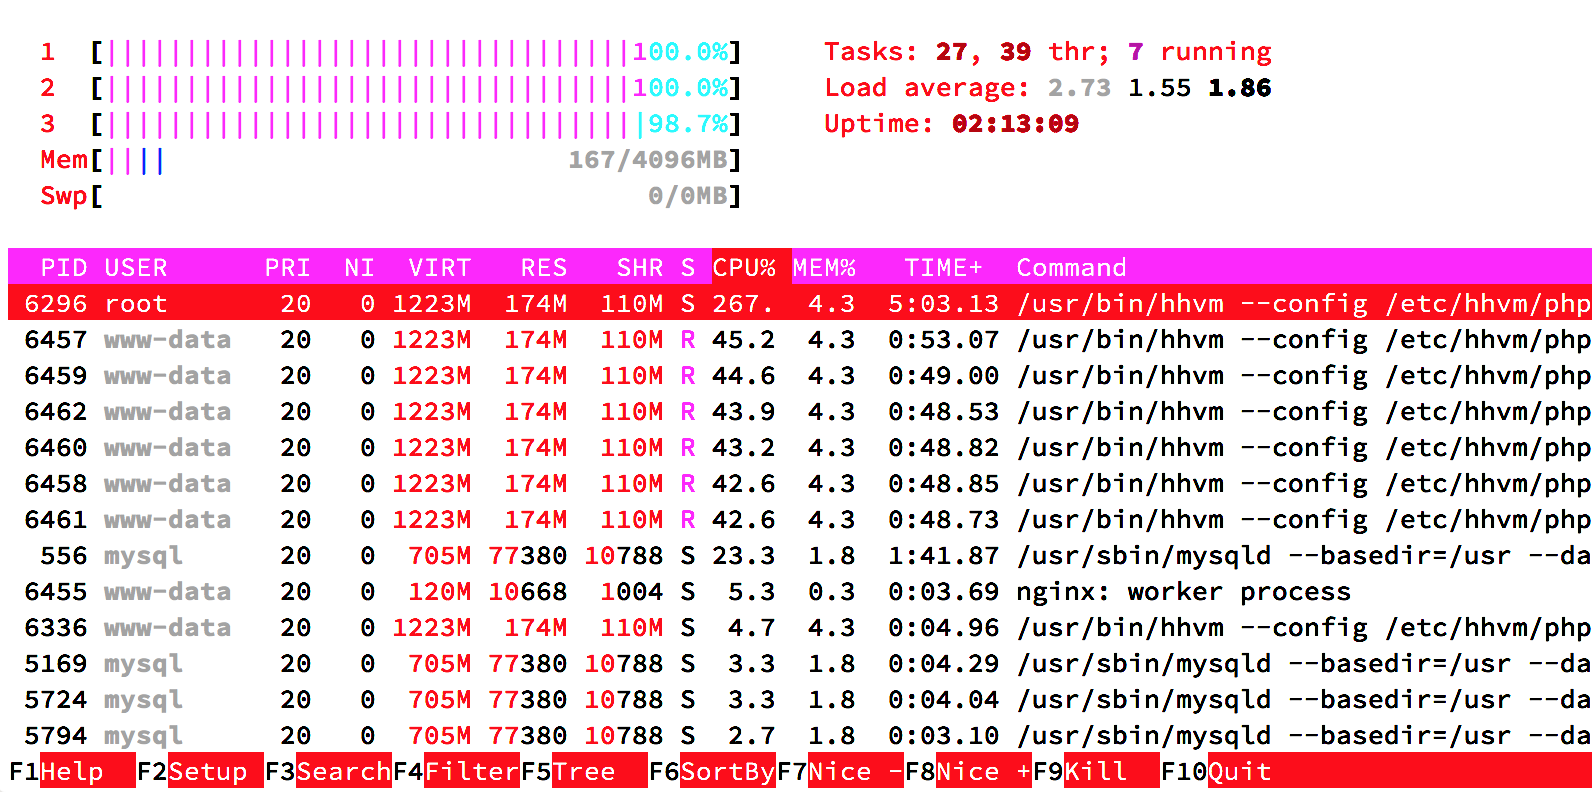
\includegraphics[scale=0.5]{figures/Nginx_HHVM_24s.png}
\caption{Nginx with HHVM: Htop process viewer 22 seconds into test}
\label{fig:nginx_hhvm_24s}
\end{center}
\end{figure}

As we can see, HHVM has much better performance profile. It can handle more requests, with less RAM usage and CPU usage. The best combination as your web serving software. 

Much higher throughput of successful requests.